\chapter{Revisão Teórica}
\graphicspath{{chapter-02/img-cap02/}}

\noindent
\section{Escoamentos Compressíveis}

Para entender o conceito de compressibilidade, \citeauthor{anderson_modern_2002} afirma que escoamento compressível é definido rotineiramente como regime de densidade variável. Essa propriedade restringe-se aos fluidos. A variação infinitesimal de densidade \(\left(d\rho\right)\) pode ser vista na equação \ref{eq:densityeq}. 

\begin{equation} \label{eq:densityeq}
    d\rho = \rho\beta dp
\end{equation}

Sob regime de altas velocidades, o gradiente de pressão \(\left(dp\right)\) costuma ser elevado, donde se conclui que a variação da densidade é elevada, portanto não pode ser desprezada. Como os gases possuem alta compressibilidade \(\left(\beta\right)\), os valores moderados a altos de variação da pressão resultam em consideráveis mudanças de densidade, tanto que esses fluidos são comumente tratados como compressíveis.

Os fundamentos dos escoamentos compressíveis são vastos para a engenharia, muito aplicados em problemas de aerodinâmica e propulsão, como é o caso do presente trabalho. Para entender os regimes de voo nos quais o projetil é submetido, deve-se considerar os três principais campos de velocidades do fluxo de ar externo: subsônico, transônico e supersônico. Todos eles dependem da propriedade termodinâmica do gás conhecida como velocidade do som ao escoamento livre \(\left(a_{\infty}\right)\), cuja relação com a velocidade do escoamento livre \(\left(U_{\infty}\right)\) é chamada de Número de Mach (M), como visto na equação \ref{eq:macheq}

\begin{equation} \label{eq:macheq}
    M = \frac{U_\infty}{a_\infty}
\end{equation}

Para os casos em que o M \(\leq\) \num{1,0} para todo o escoamento presente, define-se o regime como subsônico. Caso o regime de velocidades seja M \(\leq\) 0,8, pode-se ter certeza de que o fluido está em totalmente inserido no regime subsônico~\cite{anderson_modern_2002}. 

O regime transônico \num{0,8} \(\leq\) M \(\leq\) \num{1,2} é uma situação particular do caso anterior, porque há a formação de uma região supersônica em alguns locais. Isto significa que há energia suficiente para se desencadear ondas de choque ao longo da superfície que podem alterar consideravelmente as propriedades do fluido. A Figura \ref{fig:dali2018b} apresenta um súbito acréscimo no coeficiente de arrasto \(\left(C_D\right)\) na faixa de \num{0,8} \(\leq\) M \(\leq\) \num{1,2} em diferentes modelagens de turbulência RANS para munição \qty{122}{\millimetre} com \textit{Base Bleed} \cite{Dali2018b}.

\begin{figure}[!ht]
	\centering
    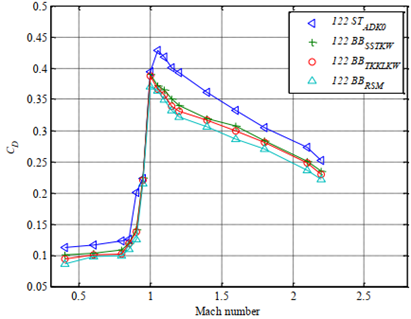
\includegraphics[width=0.5\textwidth]{foto01-dali2018b.png}
	\caption[Coeficiente de Arrasto versus Mach para o projetil com \textit{Base Bleed} pelas simulações CFD usando os modelos SST \(\kappa-\omega\), Transição \(\kappa-\kappa l-\kappa-\omega\) e RSM e comparando com resultados semi-empíricos.]{Coeficiente de Arrasto versus Mach para o projetil com \textit{Base Bleed} pelas simulações CFD usando os modelos SST \(\kappa-\omega\), Transição \(\kappa-\kappa l-\kappa-\omega\) e RSM e comparando com resultados semi-empíricos \cite{Dali2018b}.}
	\label{fig:dali2018b}
\end{figure}

O regime supersônico é válido se ao longo de todo o escoamento M \(\geq\) \num{1,0}. A onda de choque existente redireciona completamente o escoamento após esta região e o fluxo do fluido só se altera quando há o encontro com o corpo. No caso de gases, os escoamentos incompressíveis são casos especiais do regime subsônico e considerados apenas quando todo o fluxo se encontra em M \(\leq\) \num{0,3}.

Há outras formas de classificar os escoamentos, por exemplo, a partir da viscosidade. Onde os efeitos da viscosidade, condução térmica e difusividade são relevantes podemos chamar de escoamentos viscosos. A importância deste tema é considerável, tendo em vista que afeta os modelos de turbulência utilizados para compreender o arrasto de base e as técnicas para reduzi-lo. Em todos os regimes de velocidade, o ar é analisado como um meio contínuo (hipótese do \textit{continuum}), isto é, as distâncias médias entre as moléculas do gás são infinitamente menores do que o comprimento característico do escoamento.

\section{Equações de Governo}

Neste presente trabalho, as equações de Navier-Stokes são resolvidas para um fluido compressível e em regime estacionário, logo as propriedades não variam em função do tempo. Elas servem como pré-requisito para compreender o comportamento do fluido. Em todos os casos, as formulações são obtidas a partir do equilíbrio sobre um volume de controle. Para um fluido newtoniano atuando como um gás ideal, as equações de Navier-Stokes são dadas a seguir.

\subsection{Conservação de massa}

O princípio da conservação de massa indica que, na ausência de fontes e sumidouros, a região conservará a massa a nível local. O resultado disso é explicado na equação \ref{eq:gov-continuidade} \cite{Moukalled2015, Wilcox2006}.

\begin{equation}
    \label{eq:gov-continuidade}
    \frac{\partial}{\partial x_i}(\rho u_i) = 0
\end{equation}

A equação acima considera o efeito da compressibilidade, fenômeno presente no problema a ser estudado nesta pesquisa.

\subsection{Conservação do momento linear}

O princípio da conservação do momento linear indica que, na ausência de forças externas atuando sobre um corpo, o corpo retém seu momento, ou seja, o produto da massa pelo vetor velocidade. Em suma, a conservação de momento linear só é modificada na presença de uma força líquida, causada por forças de corpo e de superfície. Na forma conservativa, a conservação do momento linear é dada pela equação \ref{eq:gov-momento} \cite{Moukalled2015, Wilcox2006}

\begin{equation}
    \label{eq:gov-momento}
    \frac{\partial}{\partial x_j}(\rho u_j u_i) = -\frac{\partial p}{\partial x_i} + \frac{\partial t_{ji}}{\partial x_j}
\end{equation}

Considerando que o fluido é newtoniano, o tensor das tensões viscosas \(\left(t_{ji}\right)\) é uma função linear da taxa de deformação, demonstrado pela equação \ref{eq:tau-newtoniano}:

\begin{equation}
    \label{eq:tau-newtoniano}
    t_{ij} = \mu \left(\frac{\partial u_i}{\partial x_j} + \frac{\partial u_j}{\partial x_i} \right) + \zeta\frac{\partial u_k}{\partial x_k}\delta_{ij}
\end{equation}
%
onde \(\mu\) é a viscosidade dinâmica e \(\zeta\) é o coeficiente de dilatação da viscosidade para um gás monoatômico \(\left(\zeta = -(2/3)\mu\right)\) e \(\delta_{ij}\) é o delta de Kronecker. 

\subsection{Conservação de energia}

A conservação de energia é sustentada pela primeira lei da Termodinâmica, donde se conclui que a energia não é criada, tampouco destruída durante um processo; apenas se converte de forma (ex: energia química se transformando em energia cinética). Considerando um sistema isolado, a energia existente no processo é constante. Assumindo que o fluido é um gás ideal, a conservação de energia para escoamento compressível é definida pela equação \ref{eq:gov-energia} \cite{Moukalled2015, Wilcox2006}.

\begin{equation}
    \label{eq:gov-energia}
   \frac{\partial}{\partial x_j}\left[\rho u_j\left(h + \frac{1}{2}u_i u_i \right)\right] = \frac{\partial}{\partial x_j}\left(u_i t_{ij}\right) - \frac{\partial q_j}{\partial x_j}
\end{equation}

Para facilitar o cálculo da equação de energia, é necessário definir uma equação de estado \cite{Wilcox2006}. Assumindo o fluido de trabalho como um gás ideal, a lei dos gases perfeitos pode ser aplicada para correlacionar pressão, densidade e temperatura através da equação \ref{eq:densidade-ideal}

\begin{equation}
    \label{eq:densidade-ideal}
    \rho = \frac{p}{RT}
\end{equation}
%
cujo \(R\), presente na equação \ref{eq:densidade-ideal}, é a constante específica do gás. O termo \(h\) presente na equação \ref{eq:gov-energia} é a entalpia específica \(\left(h = e + p/\rho\right)\), cujo termo \(e\) é a energia interna específica. Por aplicar a lei dos gases perfeitos, tanto a energia interna e a entalpia específicas podem ser definidas por

\begin{equation}
	\label{eq:equacoes-entalpia-energiainterna-calores-especificos}
	e = c_{v}T \hspace{0.5cm} \text{e} \hspace{0.5cm} h = c_{p}T
\end{equation}
%
onde \(c_v\) e \(c_p\) são os calores específicos para volume e pressão constantes, respectivamente. Assumindo que o vetor de fluxo de calor é definido pela Lei de Fourier, para os gases ideais se resulta na equação \ref{eq:lei-fourier}

\begin{equation}
	\label{eq:lei-fourier}
	q_j = -c_T\frac{\partial T}{\partial x_j} = -\frac{\mu}{Pr_L}\frac{\partial h}{\partial x_j}
\end{equation}
%
sendo \(c_{T}\) a condutividade térmica do fluido e o termo \(Pr_L\) é o número de Prandtl laminar, definido por

\begin{equation}
	Pr_L = \frac{c_{p}\mu}{c_T}
\end{equation}